\section{Related Work }
% \textbf{Mixture of Experts.}
% In recent years, Large Language Models based on the Transformer architecture \cite{vaswani2023attention} have presented state-of-the-art results across many tasks and benchmarks. However, the rapid advancement in model capabilities comes at a high cost of inference and training \cite{rae2022scaling, strubell2019energy}, yielding the need for improvement of efficiency in using the computational resources. The most successful approach in this direction is Mixture-of-Experts (MoE), where each input is conditionally routed to only a part of the model paramters. In the context of Transformers, this method was proposed by \cite{shazeer2017outrageously}. Further simplifications and improvements of the technique have been applied in the architecture of Switch \cite{fedus2022switch}. More recently, \cite{zhou2022mixtureofexperts} proposed to modify the routing algorithm, achieving a better balance in the utilization of model parameters and significantly faster convergence.
%In the original formulation  it denoted an , with a separate, computationally inexpensive \textit{router model} selecting the most suitable expert.
%\subsection{}
% \paragraph{Mixture of Experts.} In the original formulation \cite{moe1991}, Mixture of Experts  was proposed as an ensemble-like architecture in which a single \textit{expert} model out of many is run for a specific input. \cite{shazeer2017outrageously} proposed to put a sparsely gated MoE layer between stacked layers of LSTM \cite{hochreiter1997long}, reaching state-of-the art results in machine translation and language modeling. In this approach, each input token was routed to a combination of experts, with the routing determined by a small gating network. 
% \paragraph{Mixture of Experts.} 
\begin{figure*}[t]
  \centering
  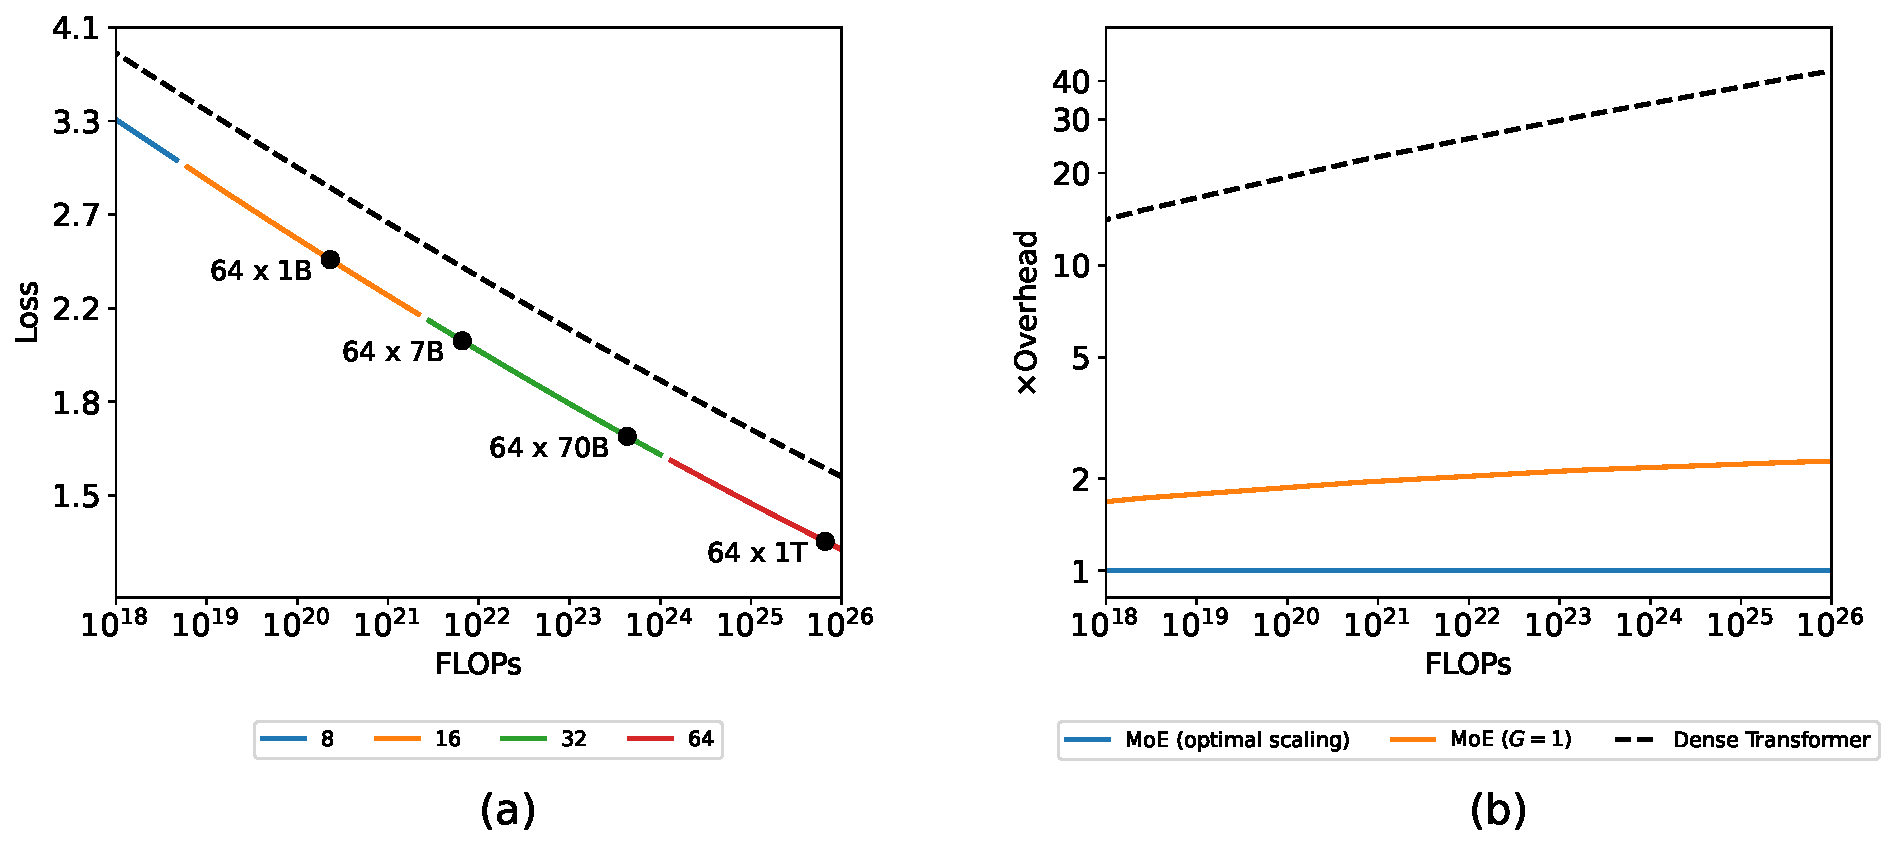
\includegraphics[width=0.99\textwidth]{figures/flags_2.pdf}
  % \medskip
  \caption{Mixture-of-Experts can be \textit{always} considered more efficient than dense Transformers, regardless of the model size. \textbf{(a)} Compute Optimal scaling curves for MoE and standard Transformers. The dashed line represents a dense Transformer. Colors denote optimal granularity for the given FLOPs training budget. \textbf{(b)} Relative number of FLOPs needed to train Transformer and Vanilla MoE (MoE with $G=1$) to achieve the performance of MoE with compute optimal $G$.}
  \label{flag_plots}
\end{figure*}
\textbf{Mixture of Experts. \ \ } 
In the context of language modeling, MoE was first introduced by \cite{shazeer2017outrageously} as a sparsely gated layer between stacked blocks of LSTM \citep{hochreiter1997long}. A similar technique was proposed in the context of Transformers by \cite{shazeer2018meshtensorflow} and \cite{lepikhin2020gshard}. \cite{fedus2022switch} proposed to route each input to only a single expert and designed a modified initialization scheme to reduce training instability.
% A similar technique was proposed in the context of Transformers by \cite{shazeer2018meshtensorflow} and \cite{lepikhin2020gshard}. These works also considered improvements in implementation and infrastructure allowing for efficient training of the gated networks. \cite{fedus2022switch} proposed to route each input to only a single expert and designed a modified initialization scheme to reduce training instability. This allowed to train models with over 1 trillion parameters and achieve 7x speedup in the pretraining speed over the dense baseline. \jk{dorzucić Artexte i tą pracę co cytuje Sebastiana}
Numerous studies have proposed to modify the original routing method. \cite{lewis2021base} used a linear assignment algorithm to postprocess token-expert mappings and ensure even expert selections. \cite{roller2021hash} suggested another approach involving deterministic hash functions. \cite{zhou2022mixtureofexperts} proposed expert choice routing, eliminating the need for additional load balancing losses. \cite{puigcerver2023sparse} designed a fully-differentiable Soft MoE architecture.


% Numerous works proposed to modify the original routing algorithm addressing its weaknesses, including load imbalance and expert under specialization. \cite{lewis2021base} used a linear assignment algorithm to postprocess token-expert mappings and ensure even expert selections. \cite{roller2021hash} suggested another approach involving deterministic hash functions. \cite{zhou2022mixtureofexperts} proposed expert choice routing instead of token choice, used originally in \cite{shazeer2017outrageously} and \cite{fedus2022switch}. This solution eliminated the need for additional load balancing losses and guaranteed balanced assignments. All of the operations used in this approach are efficiently parallelizable on modern GPU accelerators. \cite{puigcerver2023sparse} designed a fully-differentiable soft routing.
% \jk{To też można odchudzić}More recently, several open source MoE models have been released, expanding research opportunities and stimulating exploration in the community. \cite{openmoe2023} trained a 1.1T parameters model, also providing access to the intermediate checkpoints for the purpose of research. \cite{jiang2024mixtral} released Mixtral, surpassing or matching LLaMA 2 70B \cite{touvron2023llama2} and GPT-3.5 across many benchmarks. 
Concurrently to our work, \cite{dai2024deepseekmoe} proposed to modify the MoE layer by segmenting experts into smaller ones and adding shared experts to the architecture. Independently, \cite{liu2023unified} suggested a unified view of sparse \ff{} layers, considering, in particular, varying the size of memory blocks. Both approaches can be interpreted as modifying granularity.  However, we offer a comprehensive comparison of the relationship between training hyperparameters and derive principled selection criteria, which they lack.

%\sj{rephrase to state how we do better than them, not how they do worse than us. phrase us as an improvement}However, they do not present a comprehensive comparison of the relationship between training hyperparameters and lack principled selection criteria for a specific setting. \jk{druga wersja:}
%Instead, they select granularity in a rather arbitrary way.
% In the context of deep learning, MoE is built via layers that include multiple sub-networks (experts) specializing in different inputs. MoE layers gained significant popularity as an efficient way to increase the capacity of deep neural networks without increasing its inference costs, initially applied to LSTM models~\citep{shazeer2016outrageously}, and later in transformers~\citep{lepikhin2020gshard}. MoE, however, suffered from training instabilities which have been improved by selecting only one expert ~\cite{zhou2022mixture} and balancing expert load ~\cite{fedus2022switch}.  MoE models have also favorable properties in the context of the scaling laws.
% Large Language Models are widely known to benefit from high parameter count \cite{kaplan2020scaling,hoffmann2022training}, however, using all the parameters for calculating the output for each token may \mk{Czemu may, a nie po prostu result} result in unnecessarily high computational costs . In large Transformers, the \ff{} layer constitutes the majority of parameters and FLOPS and has thus become the focus of MoE-like architectural modifications. MoE in Transformer typically involves replacing the \ff{} layer with $e$ copies of itself (experts), along with a router, which handles the assignment of tokens to experts. Various 
% Most Transformer-MoEs belong to one of two categories, \textit{Token Choice} (each token is routed to a constant number of experts, e.g. \cite{shazeer2017outrageously}) or \textit{Expert Choice} (each expert receives a constant number of tokens). 
% Expert Choice (EC) is a newer technique, which achieves a better balance and faster convergence. The advantages, however, come at a price - it is not compatible with autoregressive decoding or with the batch size being different in training and inference.
% In our work, we measure the impact of granularity on autoregressive Expert Choice decoder-only models, which naturally raises the question of the applicability of the findings techniques to Token Choice architectures. We show that our findings apply to Token Choice as well, by showing that Expert Choice layers can be quickly fine-tuned to be utilized as Token Choice layers.
% MoE architectures route different inputs or parts of the input to distinct submodules. 
% 1. trochę historii i co many na myśli, 2. MoE w różnych architekturach (RNN, Transformer, etc.), 3. MoE w Transformerach - TC i EC, 4. MoE w open modelach
% \subsection{Scaling Laws}
% \paragraph{Scaling laws.} 

% \newpage
\textbf{Scaling laws.} \ Scaling laws are empirically derived equations relating the loss of a model with variables such as the number of parameters, training samples, or the computational budget. In the case of dense Transformers, scaling laws were first studied by \cite{kaplan2020scaling}, who observed power law relationships between the final model perplexity and model and dataset size. This work was extended by \cite{hoffmann2022training} by considering variable cosine cycle lengths and formulating a modified functional form of the scaling equation.
% \begin{figure*}[t]
%   \centering
%   \begin{tabular}{ c @{\hspace{30pt}} c }
%     \includegraphics[width=.43\textwidth]{icml2024/figures/plot_scaling.pdf} &
%       \includegraphics[width=.43\textwidth]{icml2024/figures/flops_save_2.pdf} \\
%     \small \textbf{(a)} &
%       \small \textbf{(b)}
%   \end{tabular}
%   \medskip
%   \caption{Mixture-of-Experts can be \textit{always} considered more efficient than dense Transformers, regardless of the model size. \textbf{(a)} Compute Optimal scaling curves for Granular models and standard Transformers. The dashed line represents a dense Transformer. Colors denote optimal granularity for the given FLOPs training budget. \textbf{(b)} Relative number of FLOPs needed to train Transformer and Vanilla MoE (MoE with $G=1$) to achieve the performance of MoE with compute optimal $G$.}
%   \label{flag_plots}
% \end{figure*}

Scaling laws have also been proposed for other architectures and training scenarios. \cite{henighan2020scaling} studied autoregressive modeling across various modalities, while \cite{ghorbani2021scaling} considered machine translation. \cite{frantar2023scaling} explored the impact of pruning on vision and language Transformers, deriving optimal sparsity for a given compute budget. \cite{clark2022unified} studied the scaling of MoE when changing model size and number of experts on a fixed dataset, concluding that routed models are more efficient only until a certain model size. In this work, we challenge that claim by considering a variable, optimal dataset size for both model families (see Section~\ref{moe_more_eff}).

% with improved scaling predictions presented in \cite{hoffmann2022training}. The extension of scaling laws to MoE-based LLMs was presented in \cite{clark2022unified}. In our work we incorporate into scaling laws granularity and the number of training tokens which allows us to achieve a better fit of the scaling laws. \jk{tu na pewno sparse scaling laws; tez inne scaling laws bylyby fajne}
%Scaling laws are of utmost practical importance, as through their extrapolation, one can justify the choice of the optimal hyperparameters of a model.
% Scaling laws have been studied in relation to MoE LLMs \cite{clark2022unified}.
% Our work differs from the previous analysis 
% %\cite{clark2022unified} 
% in the following ways:
% \begin{enumerate}
%     \item We introduce the notion of granularity and study its impact
%     \item We consider the number of training tokens 
%     \item We are more correct \sj{this needs to have better phrasing} \maciej{}
% \end{enumerate}